% Drawing 148/02-7 -- folder 148, batch 02, archive page 25 (PDF page 26).
% Transcription: croquis de la page, à l'encre, mêlés au texte. À gauche, un pantalon dont les trois bords sont notés $A$, $B$, $C$ et les six points des bords $c_B$, $c_A$, $b_C$, $b_A$, $a_C$, $a_B$, avec une flèche d'orientation ; au-dessous, un cercle sur une tige, un tore et une boucle en huit. Au centre, un graphe trivalent dont trois arêtes sont épaissies en bandes, une de ses arêtes portant une grande boucle ; le segment de $0$ à $1$ ; un ovale portant trois points. En haut à droite, un tétraèdre et une petite boucle à deux points ; à droite, une chaîne de cercles.
% Kind: plate: pair of pants with labelled boundary points, trivalent graph with ribbon thickening, small figures. Method 2 (schematic redraw from the facsimile). Status: partial.
% Notes: Schematic, from the grey render; the words and formulas of the page, which run across the sketches, are left out. Pants: three boundary ovals with the letters C (left), B (top right), A (bottom), two marked points on each (labels as the transcription gives them, placed as on the page), the three seams joining them, a circular orientation arrow in the middle. Trivalent graph: five vertices, edges as on the page, the three edges at the left vertex doubled by parallel strokes (the ribbon); the loop at the right end is drawn as on the page; the label written in the loop is unread and left out. Segment: a heavy dot 0 joined to 1, inside a pencil oval. Still differs: the tetrahedron, the chain of circles on the right edge and the figures of the bottom row are placed and shaped by eye; the long curved edges of the graph are simplified; which strokes belong to the graph and which underline the text is partly a reading. Redrawn 2026-11-12 (issue 128): to check again.
% Coordinates: 1 unit = 1 mm = 1/100 of the crop width, y downwards as on the crop (bbox in page fractions: [0.09, 0.085, 0.91, 0.52]).
% Redrawn by Claude (claude-fable-5-2), issue #128, 2026-11-12; not checked by a human; not compiled (no TeX in the session).
% Rights: reproduces part of the work -- behind RENDER_TRANSCRIPTS, never published by itself.
\documentclass[tikz,border=3pt]{standalone}
\usepackage{amsmath,amssymb}
\usetikzlibrary{patterns,arrows.meta}
\tikzset{pencil/.style={black!45}, struck/.style={black!35}, mpt/.style={circle,draw,inner sep=1.3pt}, pt/.style={circle,fill,inner sep=0.9pt}, opt/.style={circle,draw,fill=white,inner sep=1.1pt}, Rd/.style={red!75!black}, Gn/.style={green!45!black}, Br/.style={brown!70!black}}
\begin{document}
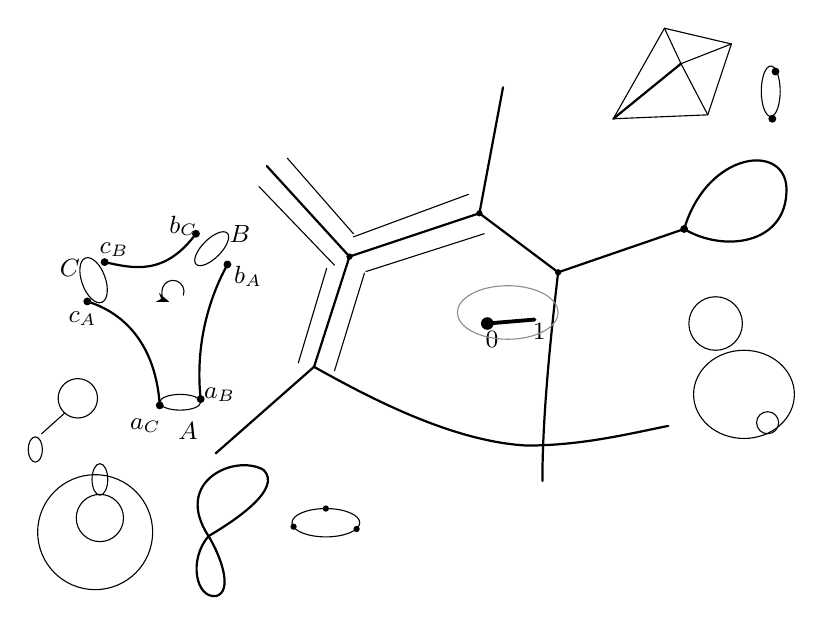
\begin{tikzpicture}[x=1mm,y=-1mm,line cap=round,line join=round,font=\small]
% pants
\draw[rotate around={20:(12,34.5)}] (12,34.5) ellipse [x radius=1.5, y radius=3];
\draw[rotate around={45:(27,30.5)}] (27,30.5) ellipse [x radius=2.8, y radius=1.2];
\draw (23,50) ellipse [x radius=2.6, y radius=1];
\draw[thick] (13.4,32.2) .. controls (17,33) and (21,34) .. (25,28.6);
\draw[thick] (29,32.5) .. controls (26,38) and (25,44) .. (25.6,49.6);
\draw[thick] (20.4,50.4) .. controls (20,44) and (17,39) .. (11.2,37.2);
\fill (13.4,32.2) circle [radius=0.5];
\fill (11.2,37.2) circle [radius=0.5];
\fill (25,28.6) circle [radius=0.5];
\fill (29,32.5) circle [radius=0.5];
\fill (20.4,50.4) circle [radius=0.5];
\fill (25.6,49.6) circle [radius=0.5];
\node at (9,33) {$C$};
\node at (30.6,28.6) {$B$};
\node at (24,53.6) {$A$};
\node at (14.6,30.6) {$c_B$};
\node at (10.6,39.4) {$c_A$};
\node at (23.4,27.6) {$b_C$};
\node at (31.6,34) {$b_A$};
\node at (18.6,53) {$a_C$};
\node at (28,49) {$a_B$};
\draw[-{Stealth[length=1.6mm]}] (23.4,36.4) arc [start angle=20, end angle=-250, radius=1.4];
% lollipop, torus, figure eight, oval with three points
\draw (10,49.5) circle [radius=2.5];
\draw (8.3,51.4) -- (5.4,54);
\draw (4.6,56) ellipse [x radius=0.9, y radius=1.6];
\draw (12.2,66.5) circle [radius=7.3];
\draw (12.8,64.7) circle [radius=3];
\draw (12.8,59.8) ellipse [x radius=1, y radius=2];
\draw[thick] (26.6,67) .. controls (22,60) and (30,56.5) .. (33.6,58.6) .. controls (36,61) and (30,65) .. (26.6,67) .. controls (24,70) and (25,75) .. (27.6,74.6) .. controls (29.6,74) and (28.4,70) .. (26.6,67);
\draw (41.5,65.3) ellipse [x radius=4.3, y radius=1.8];
\fill (37.4,65.8) circle [radius=0.4];
\fill (41.5,63.5) circle [radius=0.4];
\fill (45.4,66.1) circle [radius=0.4];
% trivalent graph
\coordinate (u) at (44.5,31.5);
\coordinate (v) at (61,26);
\coordinate (w) at (71,33.5);
\coordinate (x) at (40,45.5);
\coordinate (z) at (87,28);
\draw[thick] (u) -- (34,20);
\draw[thick] (u) -- (x);
\draw[thick] (u) -- (v);
\draw[thick] (v) -- (64,10);
\draw[thick] (v) -- (w);
\draw[thick] (w) -- (z);
\draw[thick] (w) .. controls (70,42) and (69,52) .. (69,60);
\draw[thick] (x) -- (27.5,56.5);
\draw[thick] (x) .. controls (48,50) and (58,55) .. (67,55.5) .. controls (74,55.5) and (80,54) .. (85,53);
\draw[thick] (z) .. controls (90,18) and (100,17) .. (100,23) .. controls (100,30) and (92,31) .. (z);
\fill (u) circle [radius=0.4];
\fill (v) circle [radius=0.4];
\fill (w) circle [radius=0.4];
\fill (z) circle [radius=0.5];
% ribbon strokes along the three edges at u
\draw (33,22.6) -- (42.6,32.6);
\draw (36.6,19) -- (45,28.6);
\draw (41.6,33) -- (38,45);
\draw (46.4,33.6) -- (42.6,46);
\draw (45,29) -- (59.6,23.6);
\draw (46.6,33.4) -- (61.6,28.6);
% segment 0--1
\fill (62,40) circle [radius=0.8];
\draw[line width=1.4pt] (62,40) -- (68,39.5);
\node at (62.6,42) {$0$};
\node at (68.6,41) {$1$};
\draw[pencil] (64.6,38.6) ellipse [x radius=6.4, y radius=3.4];
% tetrahedron
\coordinate (p) at (84.5,2.5);
\coordinate (q) at (93,4.5);
\coordinate (r) at (78,14);
\coordinate (s) at (90,13.5);
\coordinate (t) at (86.6,7);
\draw (p) -- (q) -- (s) -- (r) -- cycle;
\draw (p) -- (t);
\draw (q) -- (t);
\draw[thick] (r) -- (t);
\draw (s) -- (t);
% small loop with two points, chain of circles
\draw (98,10.5) ellipse [x radius=1.2, y radius=3.2];
\fill (98.6,8) circle [radius=0.5];
\fill (98.2,14) circle [radius=0.5];
\draw (91,40) circle [radius=3.4];
\draw (94.6,49) ellipse [x radius=6.4, y radius=5.6];
\draw (97.6,52.6) circle [radius=1.4];
\end{tikzpicture}
\end{document}
